\documentclass[8pt,pdf,hyperref={unicode},serif]{beamer}

\usepackage{amsfonts}
\usepackage{amsmath}
\usepackage{amssymb}
\usepackage{booktabs} %пакет для использования \specialrule{}{}{} в \tabular{}{}
\usepackage{caption}
\usepackage{cite} 
\usepackage{color}
\usepackage{delarray}
\usepackage{enumerate}
\usepackage{fancyhdr} 
\usepackage{float}
\usepackage{indentfirst} %отступ в первом абзаце любого раздела
\usepackage{mathtext}
\usepackage[section]{placeins}
\usepackage{textcomp}
\usepackage{upgreek}
\usepackage{wrapfig}

\usepackage[english,russian]{babel}
\usepackage[utf8]{inputenc} %чтобы можно было набирать русский текст
\usepackage[T2A]{fontenc} %кодировка текстовых шрифтов с поддержкой кириллических букв
\usepackage{cmap}
\usepackage{listingsutf8} 

\graphicspath{{./images/}}
\usepackage{svg}
\renewcommand{\theequation}{\arabic{section}.\arabic{equation}}
\setsvg{inkscape = inkscape -z -D}
\setsvg{svgpath = images/}
\usepackage{epstopdf}

% отключить клавиши навигации
\setbeamertemplate{navigation symbols}{}

% тема оформления
\usetheme{CambridgeUS}

% цветовая схема
\usecolortheme{seahorse}

\title{Численное моделирование ускорения частиц на ударных волнах } % заголовок
\author{Антон Лиознов} % авторы
\date{22 июня 2015} % день (сегодня)
\institute{Санкт-Петербургский Политехнический Университет имени Петра Великого \\ кафедра космических исследований.\\
    \vspace{0.7cm}
    Научный руководитель:  Гладилин Пётр Евгеньевич \\ н.с. ФТИ им. А.Ф.Иоффе, к.ф.-м.н.
    \vspace{0.7cm}
}
\AtBeginSection[] % как ясно из названия, перед каждой секцией вставляем что написано
{
  \begin{frame}{Содержание}
  \tableofcontents[currentsection,hideallsubsections]
  \end{frame}
}
\begin{document}
\begin{frame}
\titlepage 
\end{frame} 
\begin{frame}
\tableofcontents[hideallsubsections] % автоматом получаем содержание (скрываем подсекции)
\end{frame}
\section{Введение}
\begin{frame}{Физика процесса}
\begin{figure}[H]
\center
\includesvg[width=0.60\linewidth]{lamin}
\caption{Ускорение на ударных волнах при ламинарном (а) и турбулентном(б) движении.}
\end{figure}
 
\begin{equation}
n \sim p^{-\gamma}
\end{equation}
 с показателем $\gamma=\frac{\sigma+2}{\sigma-1}$
\end{frame}

\begin{frame}{Исследования}
\begin{itemize}
\item 70-80 гг прошлого века - Аксворд, Лиир, Скадрон, Белл, Крымский, Бережко, Бландфолд, Острикер -- теоретическое исследование проблемы ускорения на ударных волнах
\item 1992 г - Ахтенберг и Круллс - моделирование с использованием стохастического подхода
\item 2011 г - Канг - моделирование с использованием решения разностной схемы
\pause
~\\
\item Никто из авторов не делал сравнения с точки зрения времени работы и расширяемости.
\end{itemize}
\end{frame}
\section{Цели и задачи}
\begin{frame}{Цели и задачи}
\textit{\texttt{Цель:}} анализ и сравнение 
диффузиозно-конвективного и стохастического подхода в ускорении частиц на ударных волнах.

\textit{\texttt{Задачи:}}
\begin{enumerate}
\item Реализовать численное моделирование решения диффузиозно-конвективного уравнения ускорения частиц на ударных волнах с помощью решения \texttt{разностной схемы}
\item Реализовать численное моделирование ускорения частиц на ударных волнах \texttt{стохастическим} методом.
\item Провести \texttt{сравнение} данных подходов
\item Указать \texttt{положительные и отрицательные} стороны в каждом из них
\end{enumerate}
\end{frame}

\section{Методы}
\begin{frame}{методы}
\framesubtitle{неявный метод Эйлера}
Изначальное уравнение имеет вид
\begin{equation}
\frac{\partial f}{\partial t} = \frac{\partial}{\partial x} \kappa \frac{\partial f}{\partial x} - u \frac{\partial f}{\partial x} - \frac{du}{3dx} \delta(x) p \frac{\partial f}{\partial p} +Q
\end{equation}

\pause
Разностная схема
\begin{multline}
\frac{f_{i,j,k} - f_{i,j,k-1}}{\Delta t} = \kappa_{j} \frac{f_{i+1,j,k}+f_{i-1,j,k}-2f_{i,j,k}}{\Delta^2 x} \\
- u_i\frac{f_{i,j,k}-f_{i-1,j,k}}{\Delta x}-\frac{u_i-u_{i-1}}{3\Delta x}\frac{f_{i,j,k}-f_{i,j-1,k}}{\Delta y} + Q
\end{multline}
\pause
\begin{itemize}
\item решение трёхдиагональной матрицы методом прогонки
\item язык C++
\end{itemize}
\end{frame}

\begin{frame}{методы}
\framesubtitle{стохастический метод}
Уравнением в виде Фоккера-Планка
\begin{equation}
\frac{\partial F(\vec{Z}, t)}{\partial t} = \frac{\partial}{\partial \vec{Z}}\left( -\dot{\vec{Z}}F+\frac{\partial}{\partial\vec{Z}}[DF]  \right)
\end{equation}
\pause
Общий вид уравнения:
\begin{equation}
dx = a(x, t)dt + b(x,t) \underbrace{\varepsilon \sqrt{dt}}_{dW}
\end{equation}
\pause
В форме уравнения Ито:
\begin{equation}
d\vec{Z} = d\dot{\vec{Z}}(\vec{Z}, t)+\sqrt{2D}dW
\end{equation}
В приложении к задаче:
\begin{eqnarray}
dx = V(x)dt+\sqrt{2K_{\parallel}}dW\\
du = - \frac{1}{3} \frac{\partial V}{\partial x} dt
\end{eqnarray}
\pause
 язык C++ и Python
\end{frame}

\begin{frame}
\begin{figure}[H]
  \centering
  \includesvg[width=0.70\linewidth]{principle}
  \caption{Последовательность итераций для разностной схемы (слева) и стохастического подхода(справа)}
\end{figure}
\end{frame}

\section{Результаты}
\begin{frame}{Результаты}
\begin{columns}
\begin{column}{0.5\textwidth}
Эйлер
\begin{figure}[H]
\centering
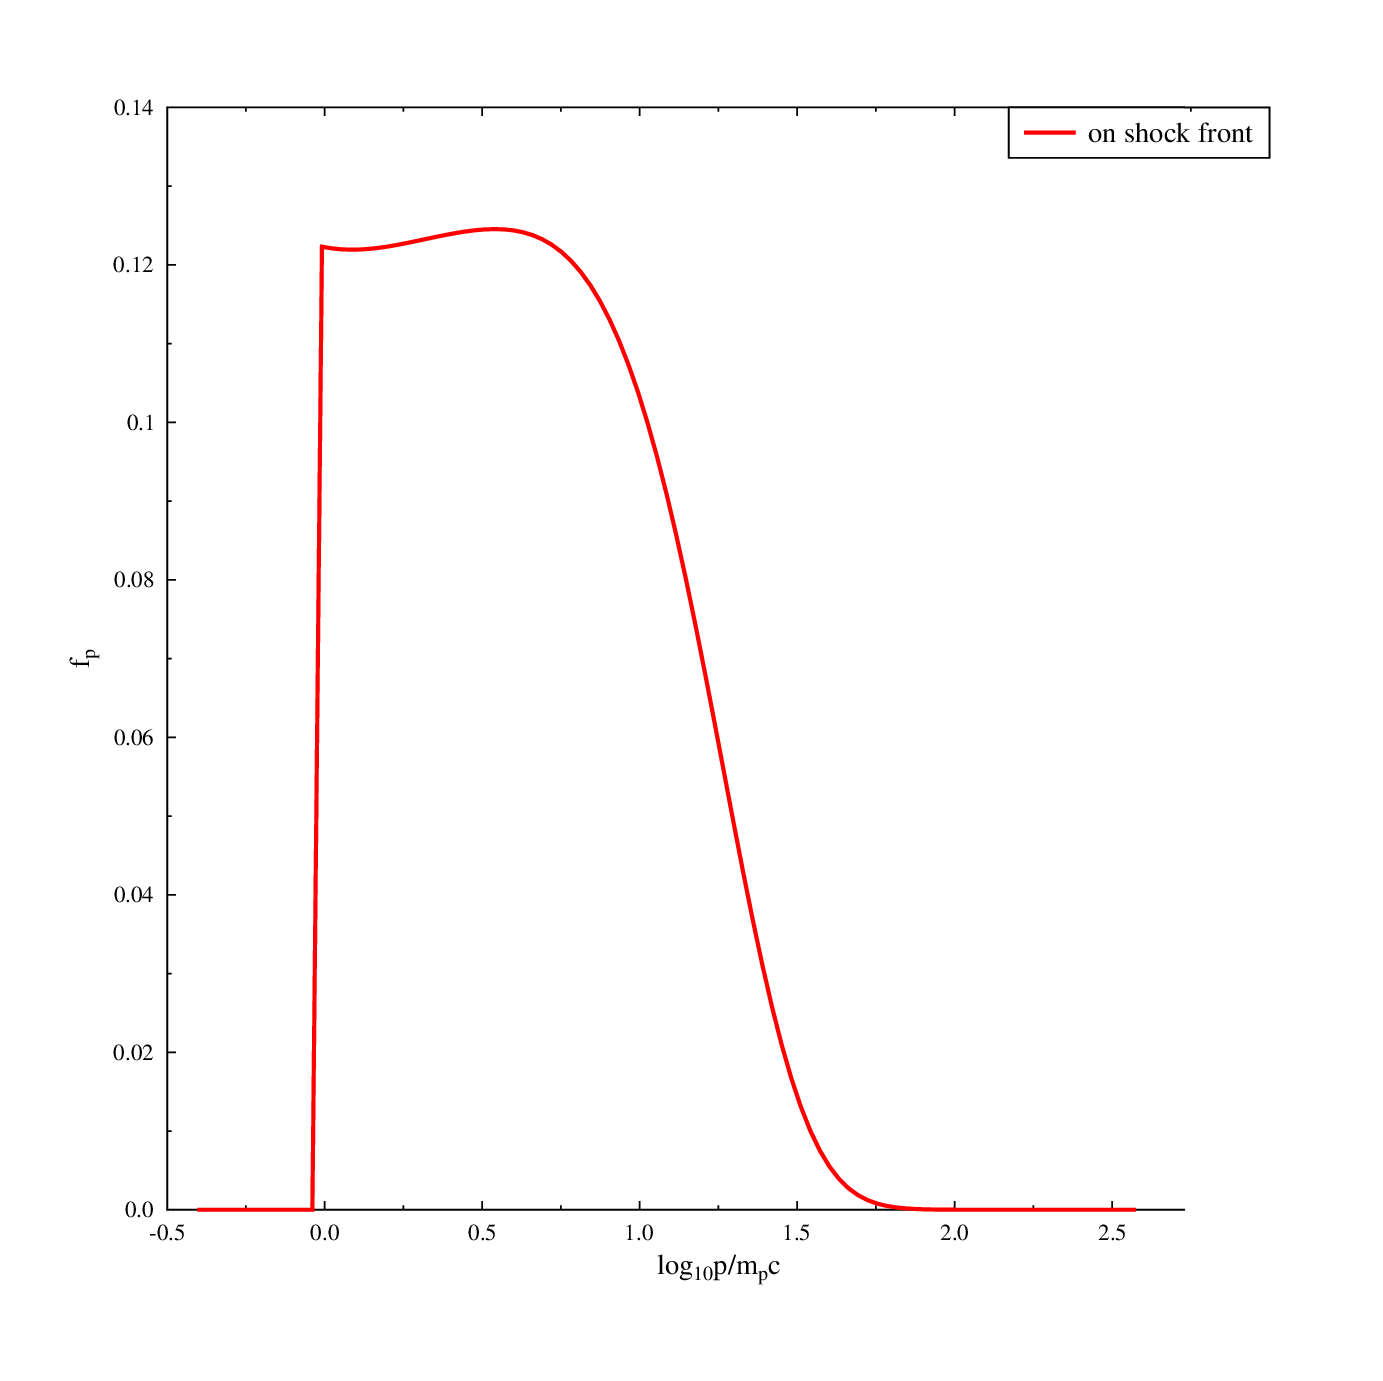
\includegraphics[width=0.90\linewidth]{r_common}
\caption{Пример запуска программы решения с разностной схемой}
\end{figure}
\end{column}

\begin{column}{0.5\textwidth}
Стохастика
\begin{figure}[H]
\centering
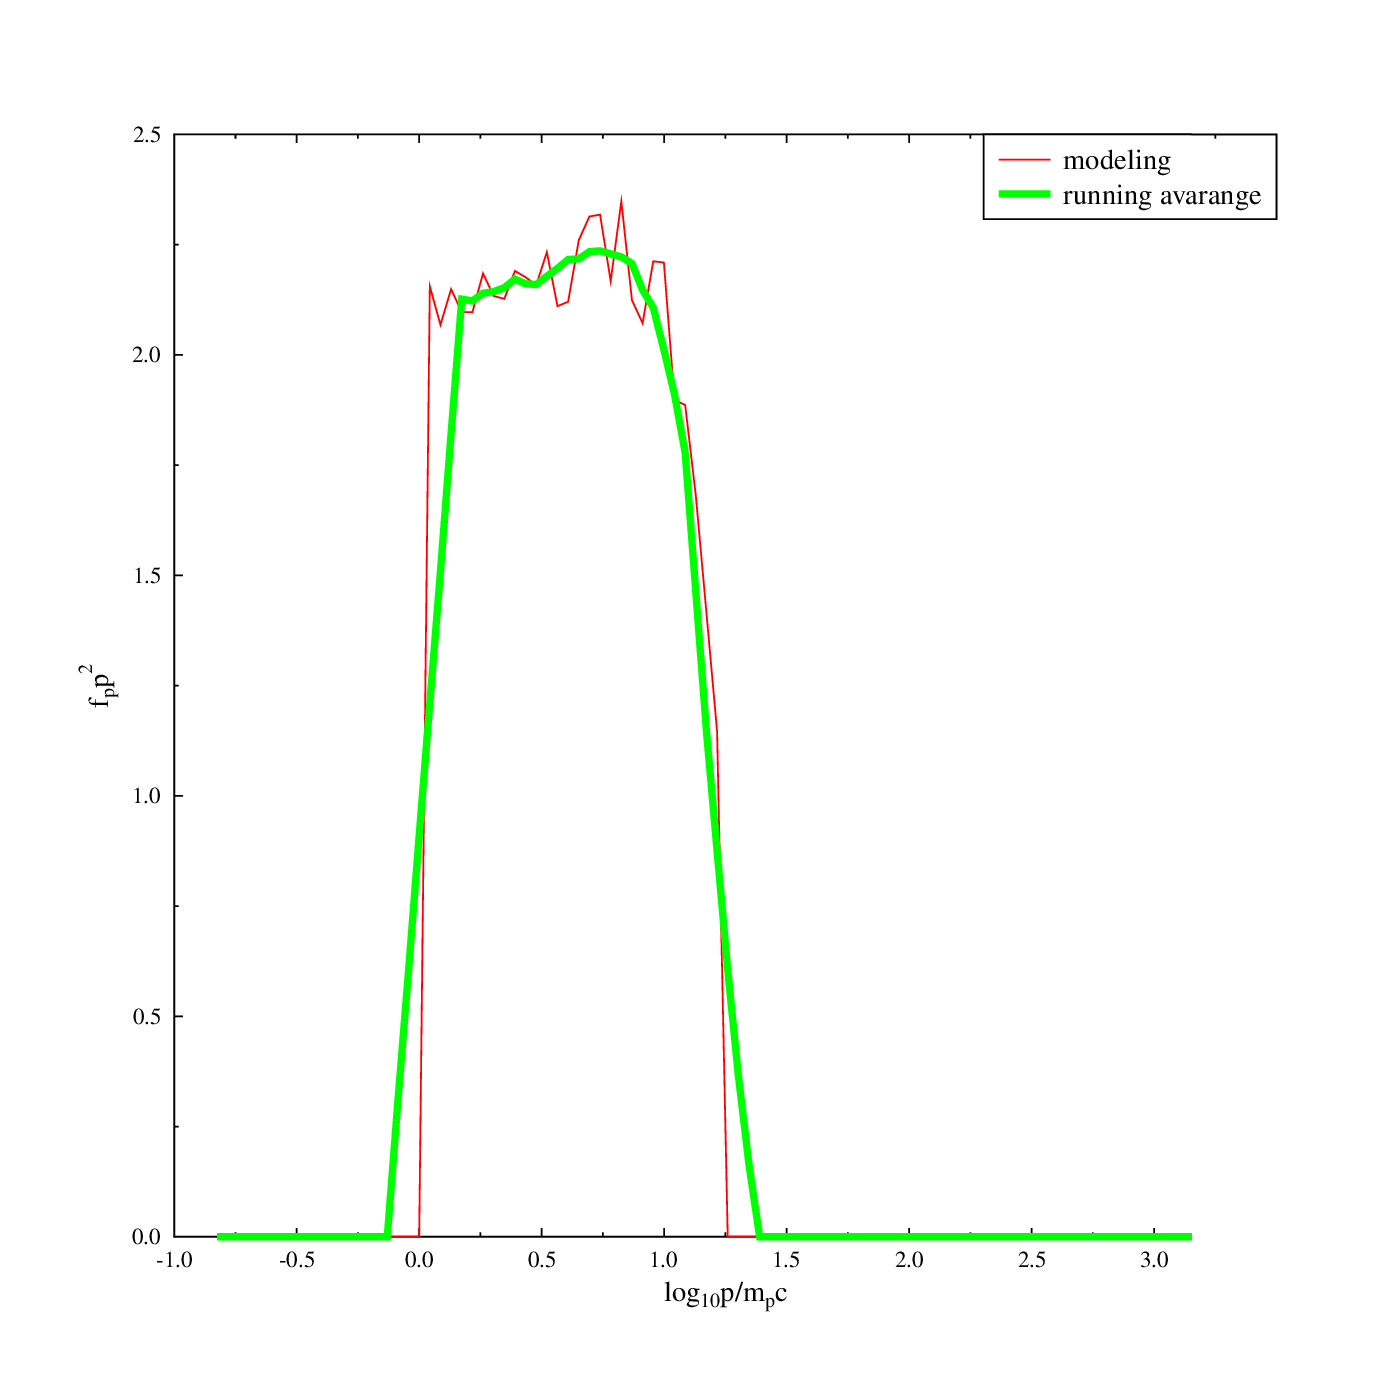
\includegraphics[width=0.90\linewidth]{stoh_bom_one}
\caption{Пример запуска программы решения стохастическим методом}
\end{figure}
\end{column}
\end{columns}
\end{frame}


\begin{frame}{Результаты}
\framesubtitle{время выполнения}
\begin{columns}
\begin{column}{0.5\textwidth}
Эйлер
\begin{figure}[H]
\centering
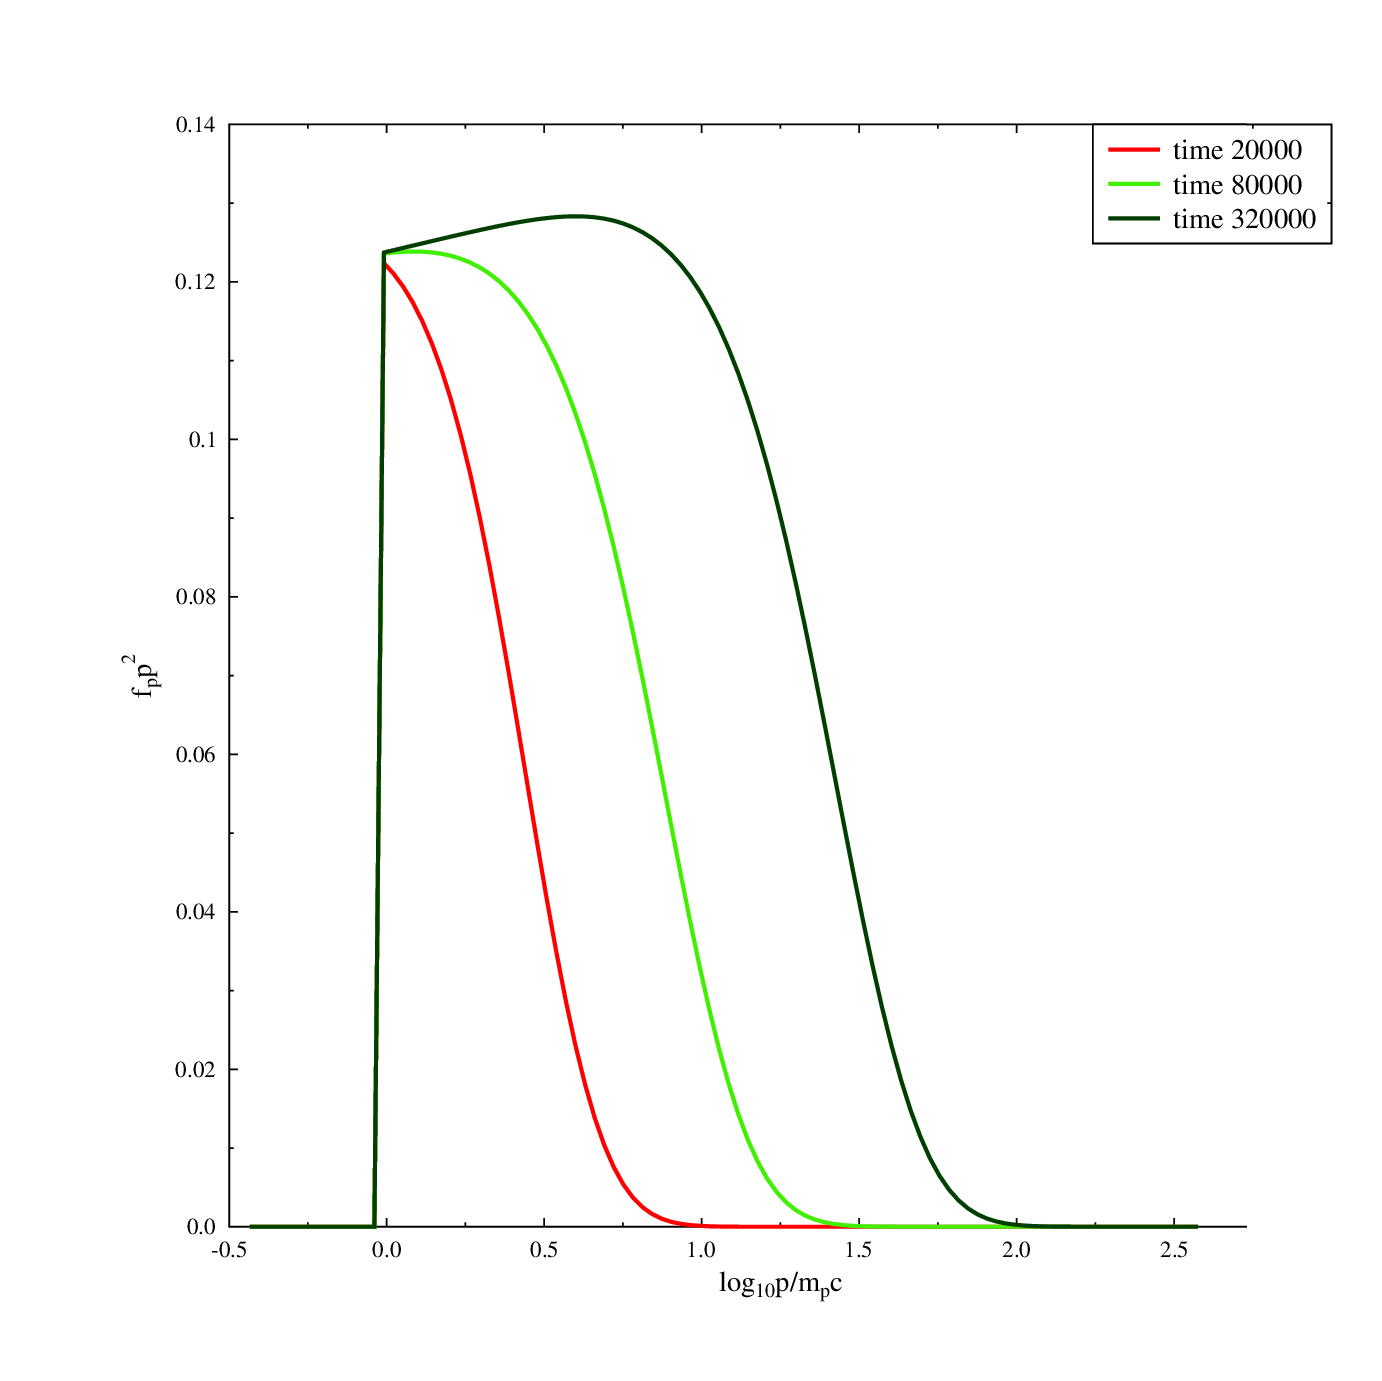
\includegraphics[width=0.90\linewidth]{r_times}
\caption{Различные времена запуска}
\end{figure}
\end{column}

\begin{column}{0.5\textwidth}
Стохастика
\begin{figure}[H]
\centering
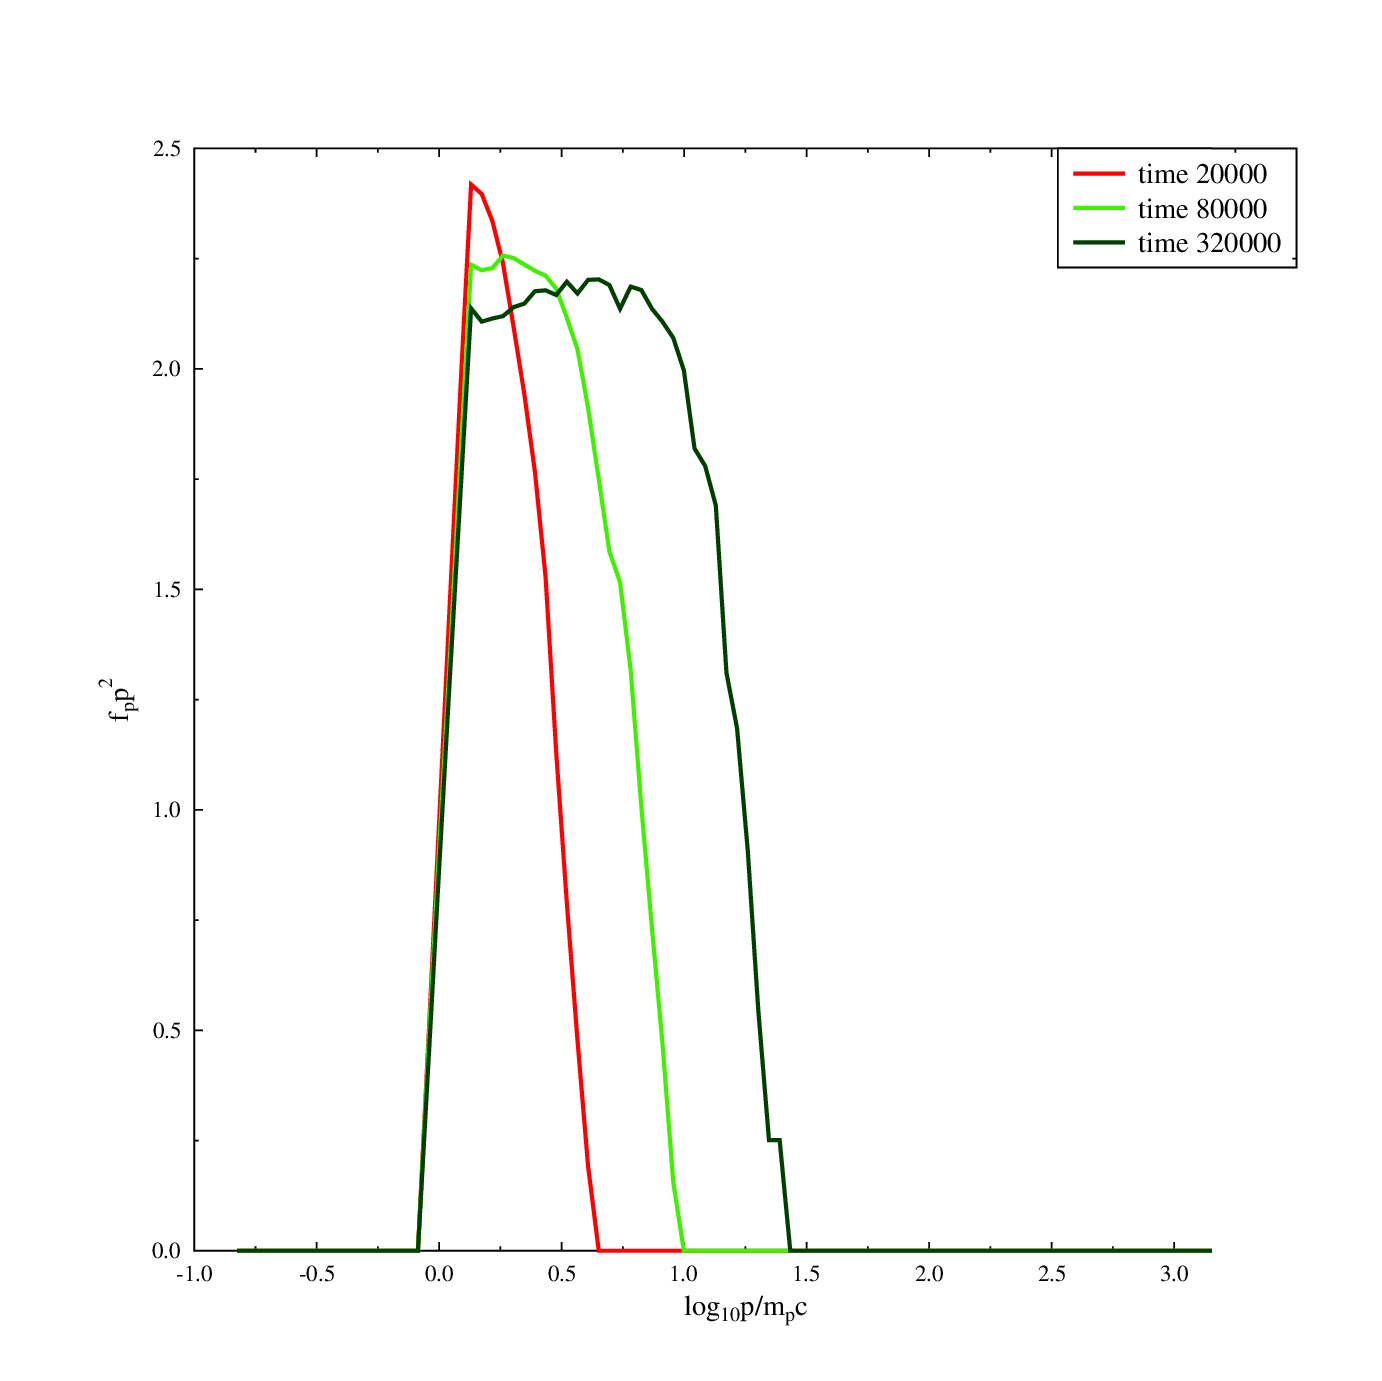
\includegraphics[width=0.90\linewidth]{stoh_times}
\caption{Различные времена запуска}
\end{figure}
\end{column}
\end{columns}
\end{frame}


\begin{frame}{Результаты}
\framesubtitle{"высота" графика}
\begin{columns}
\begin{column}{0.5\textwidth}
Эйлер
\begin{figure}[H]
\centering
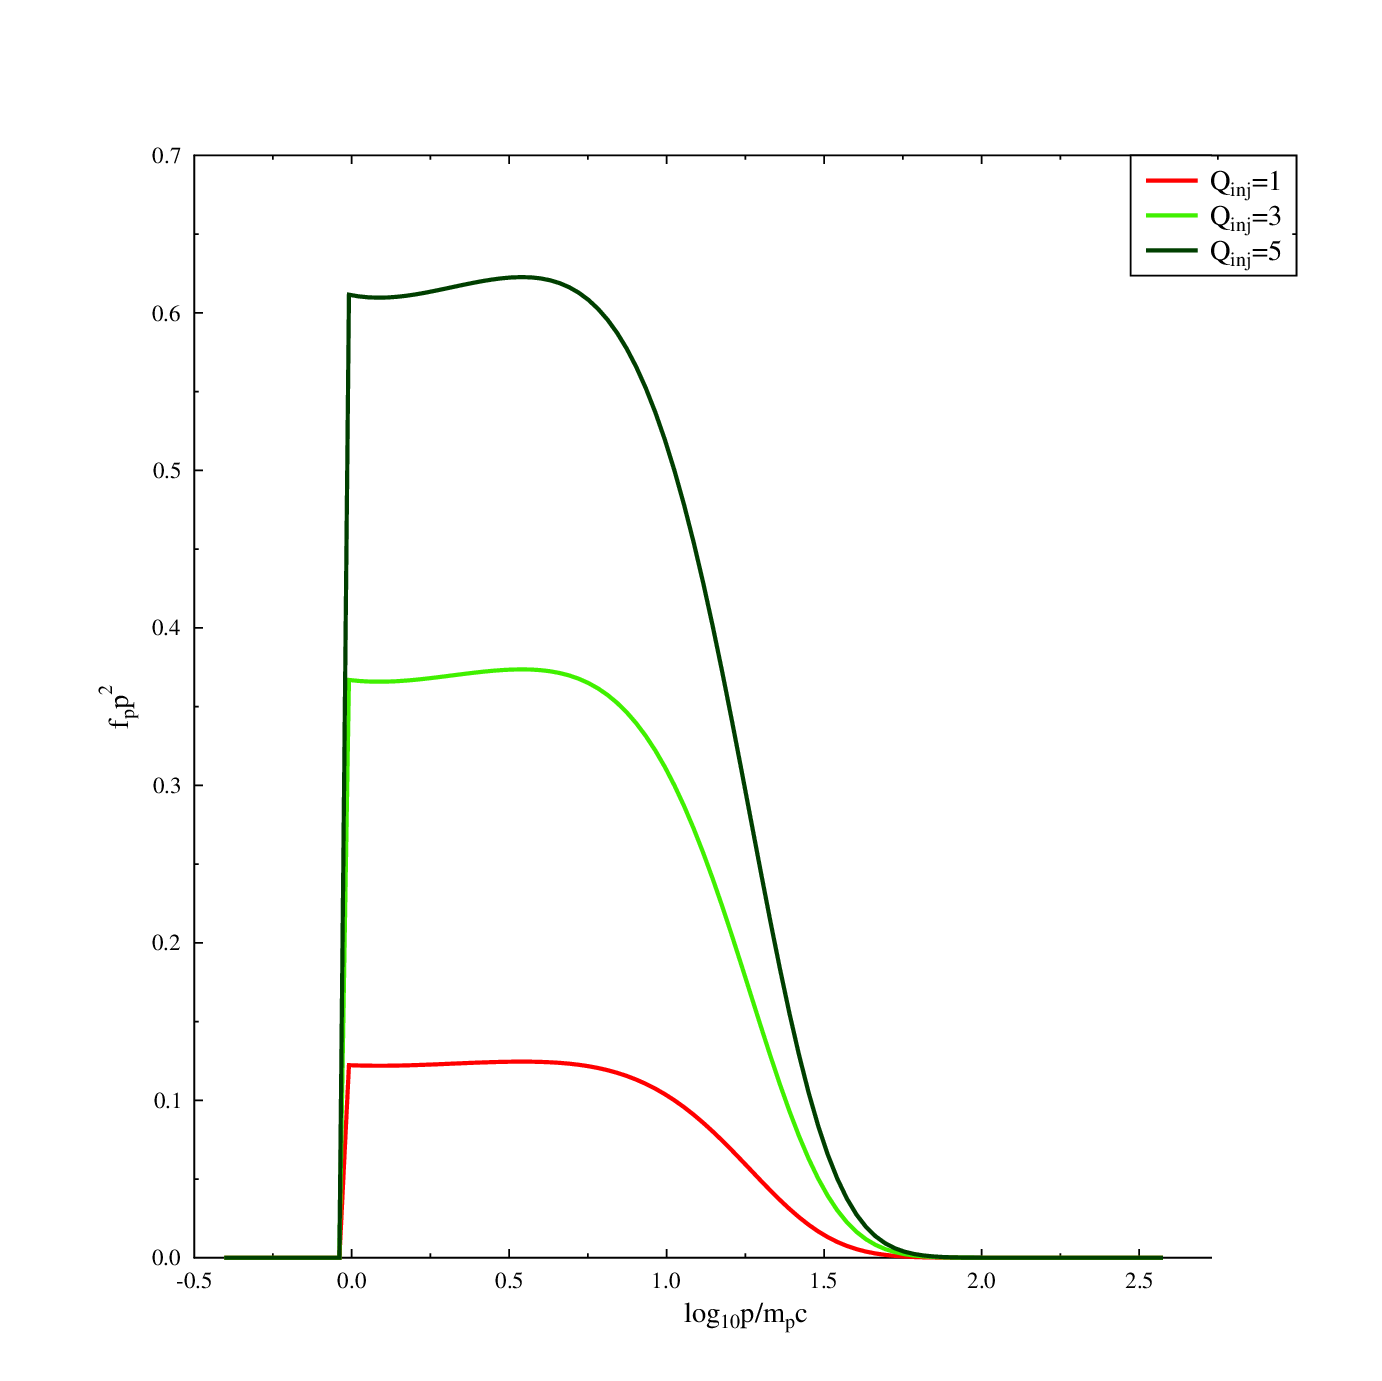
\includegraphics[width=0.90\linewidth]{r_Qinj}
\caption{различные мощности инжекции}
\end{figure}
\end{column}

\begin{column}{0.5\textwidth}
Стохастика
\begin{figure}[H]
\centering
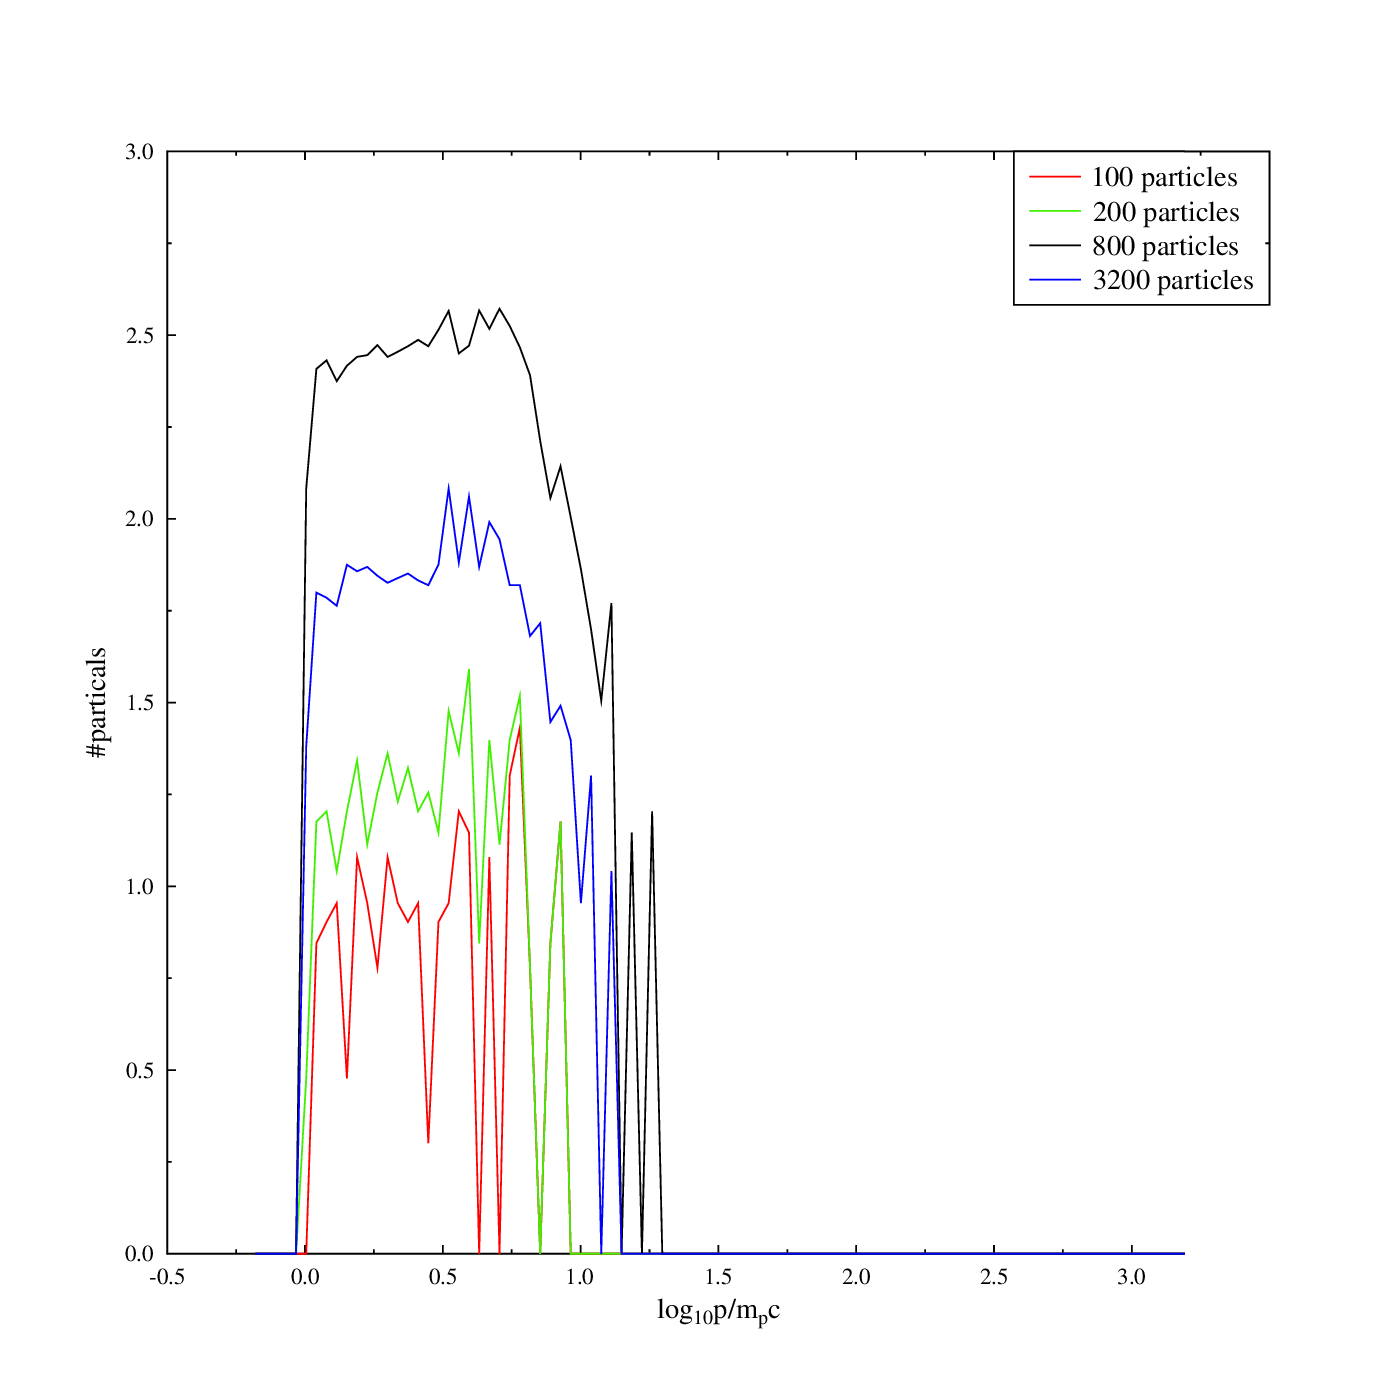
\includegraphics[width=0.90\linewidth]{stoh_particles}
\caption{различное количество частиц}
\end{figure}
\end{column}
\end{columns}
\end{frame}


\begin{frame}{Результаты}
\framesubtitle{виды коэффициента диффузии}
\begin{columns}
\begin{column}{0.5\textwidth}
Эйлер
\begin{figure}[H]
\centering
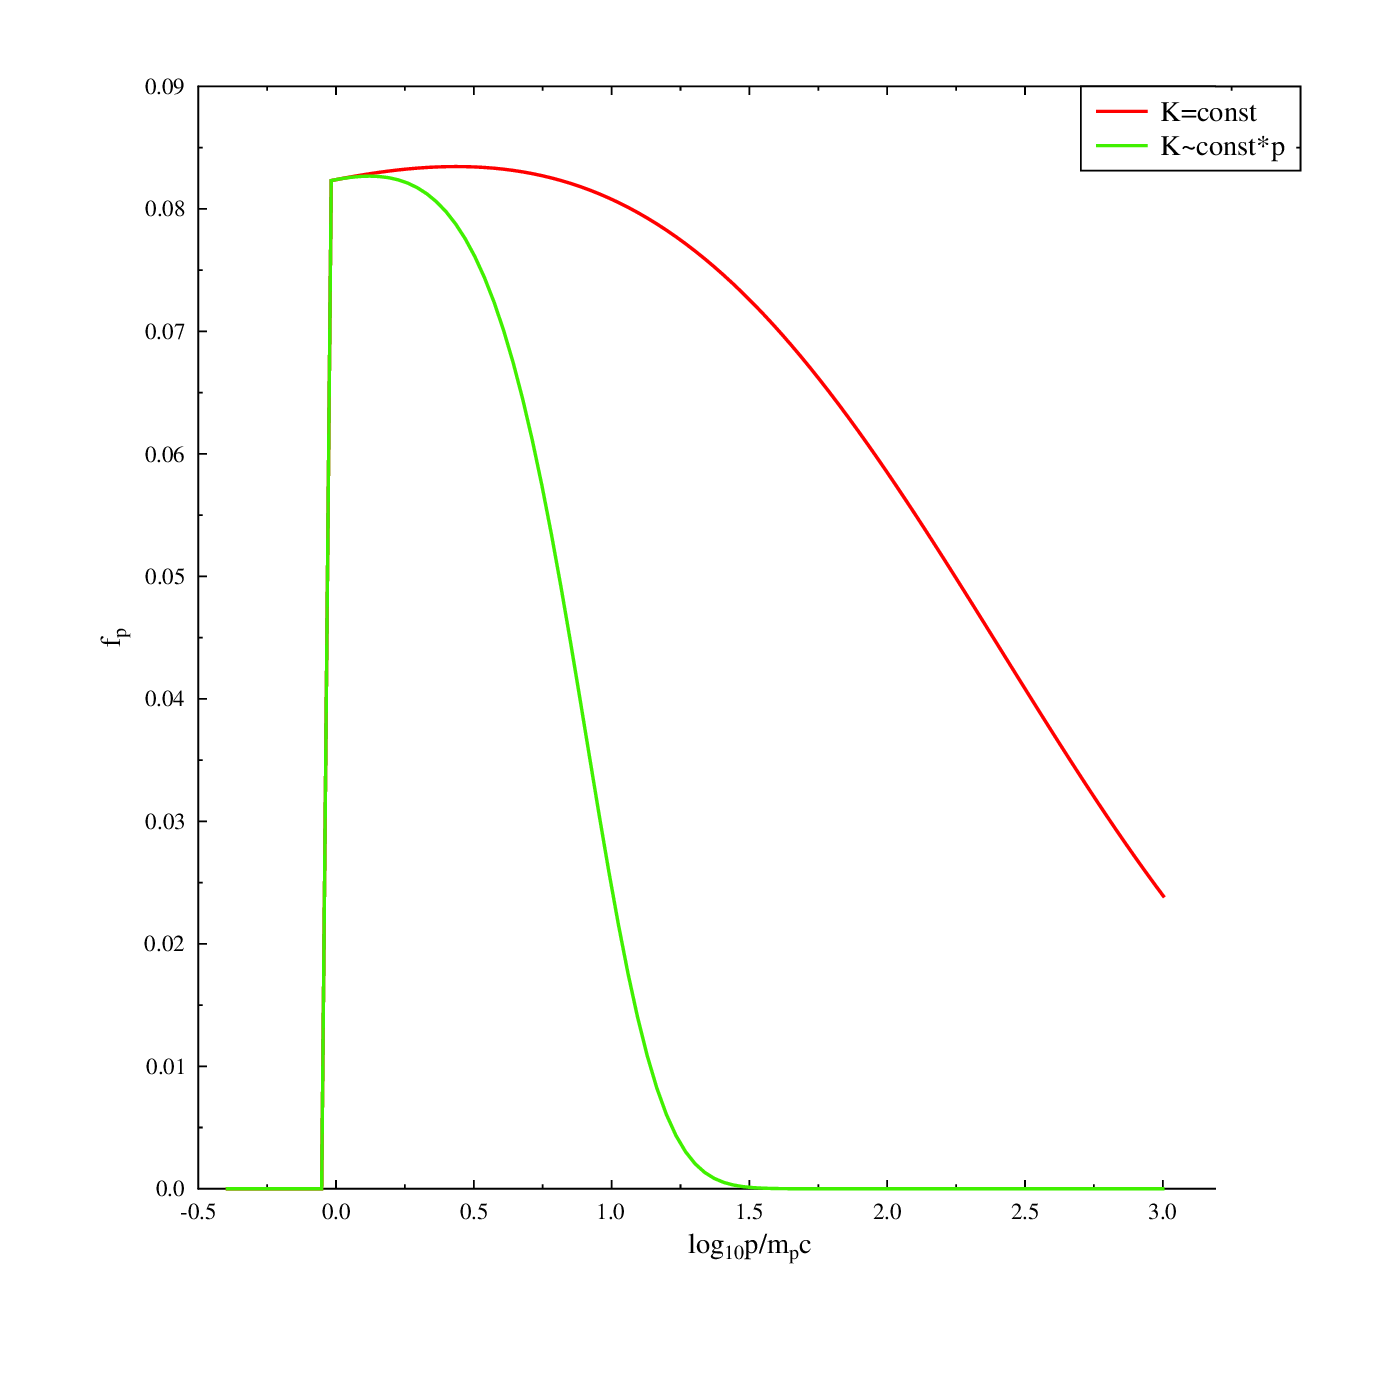
\includegraphics[width=0.90\linewidth]{r_bom_or_not2}
\caption{различные коэффициенты диффузии}
\end{figure}
\end{column}

\begin{column}{0.5\textwidth}
Стохастика
\begin{figure}[H]
\centering
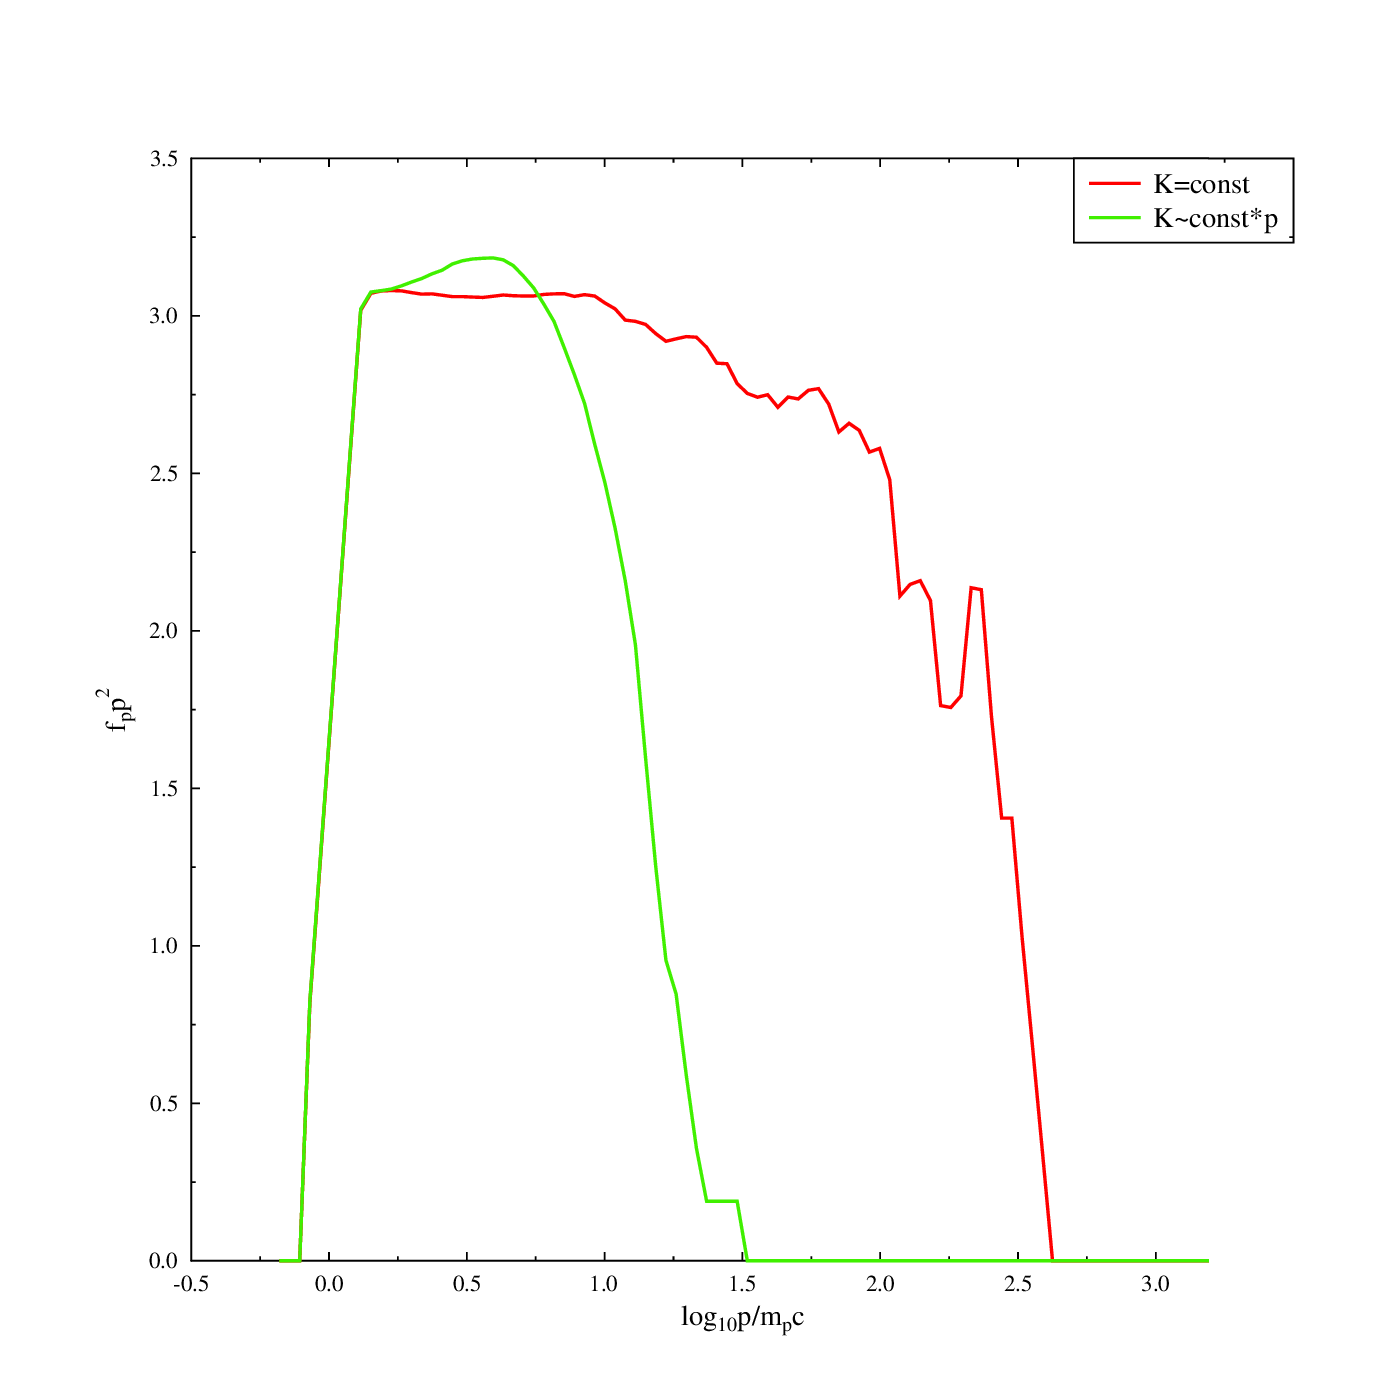
\includegraphics[width=0.90\linewidth]{stoh_bom_or_not}
\caption{различные коэффициенты диффузии}
\end{figure}
\end{column}
\end{columns}
\end{frame}


\begin{frame}{Результаты}
\framesubtitle{дополнительные результаты для стохастического подхода}
\begin{columns}
\begin{column}{0.5\textwidth}
Стохастика
\begin{figure}[H]
\centering
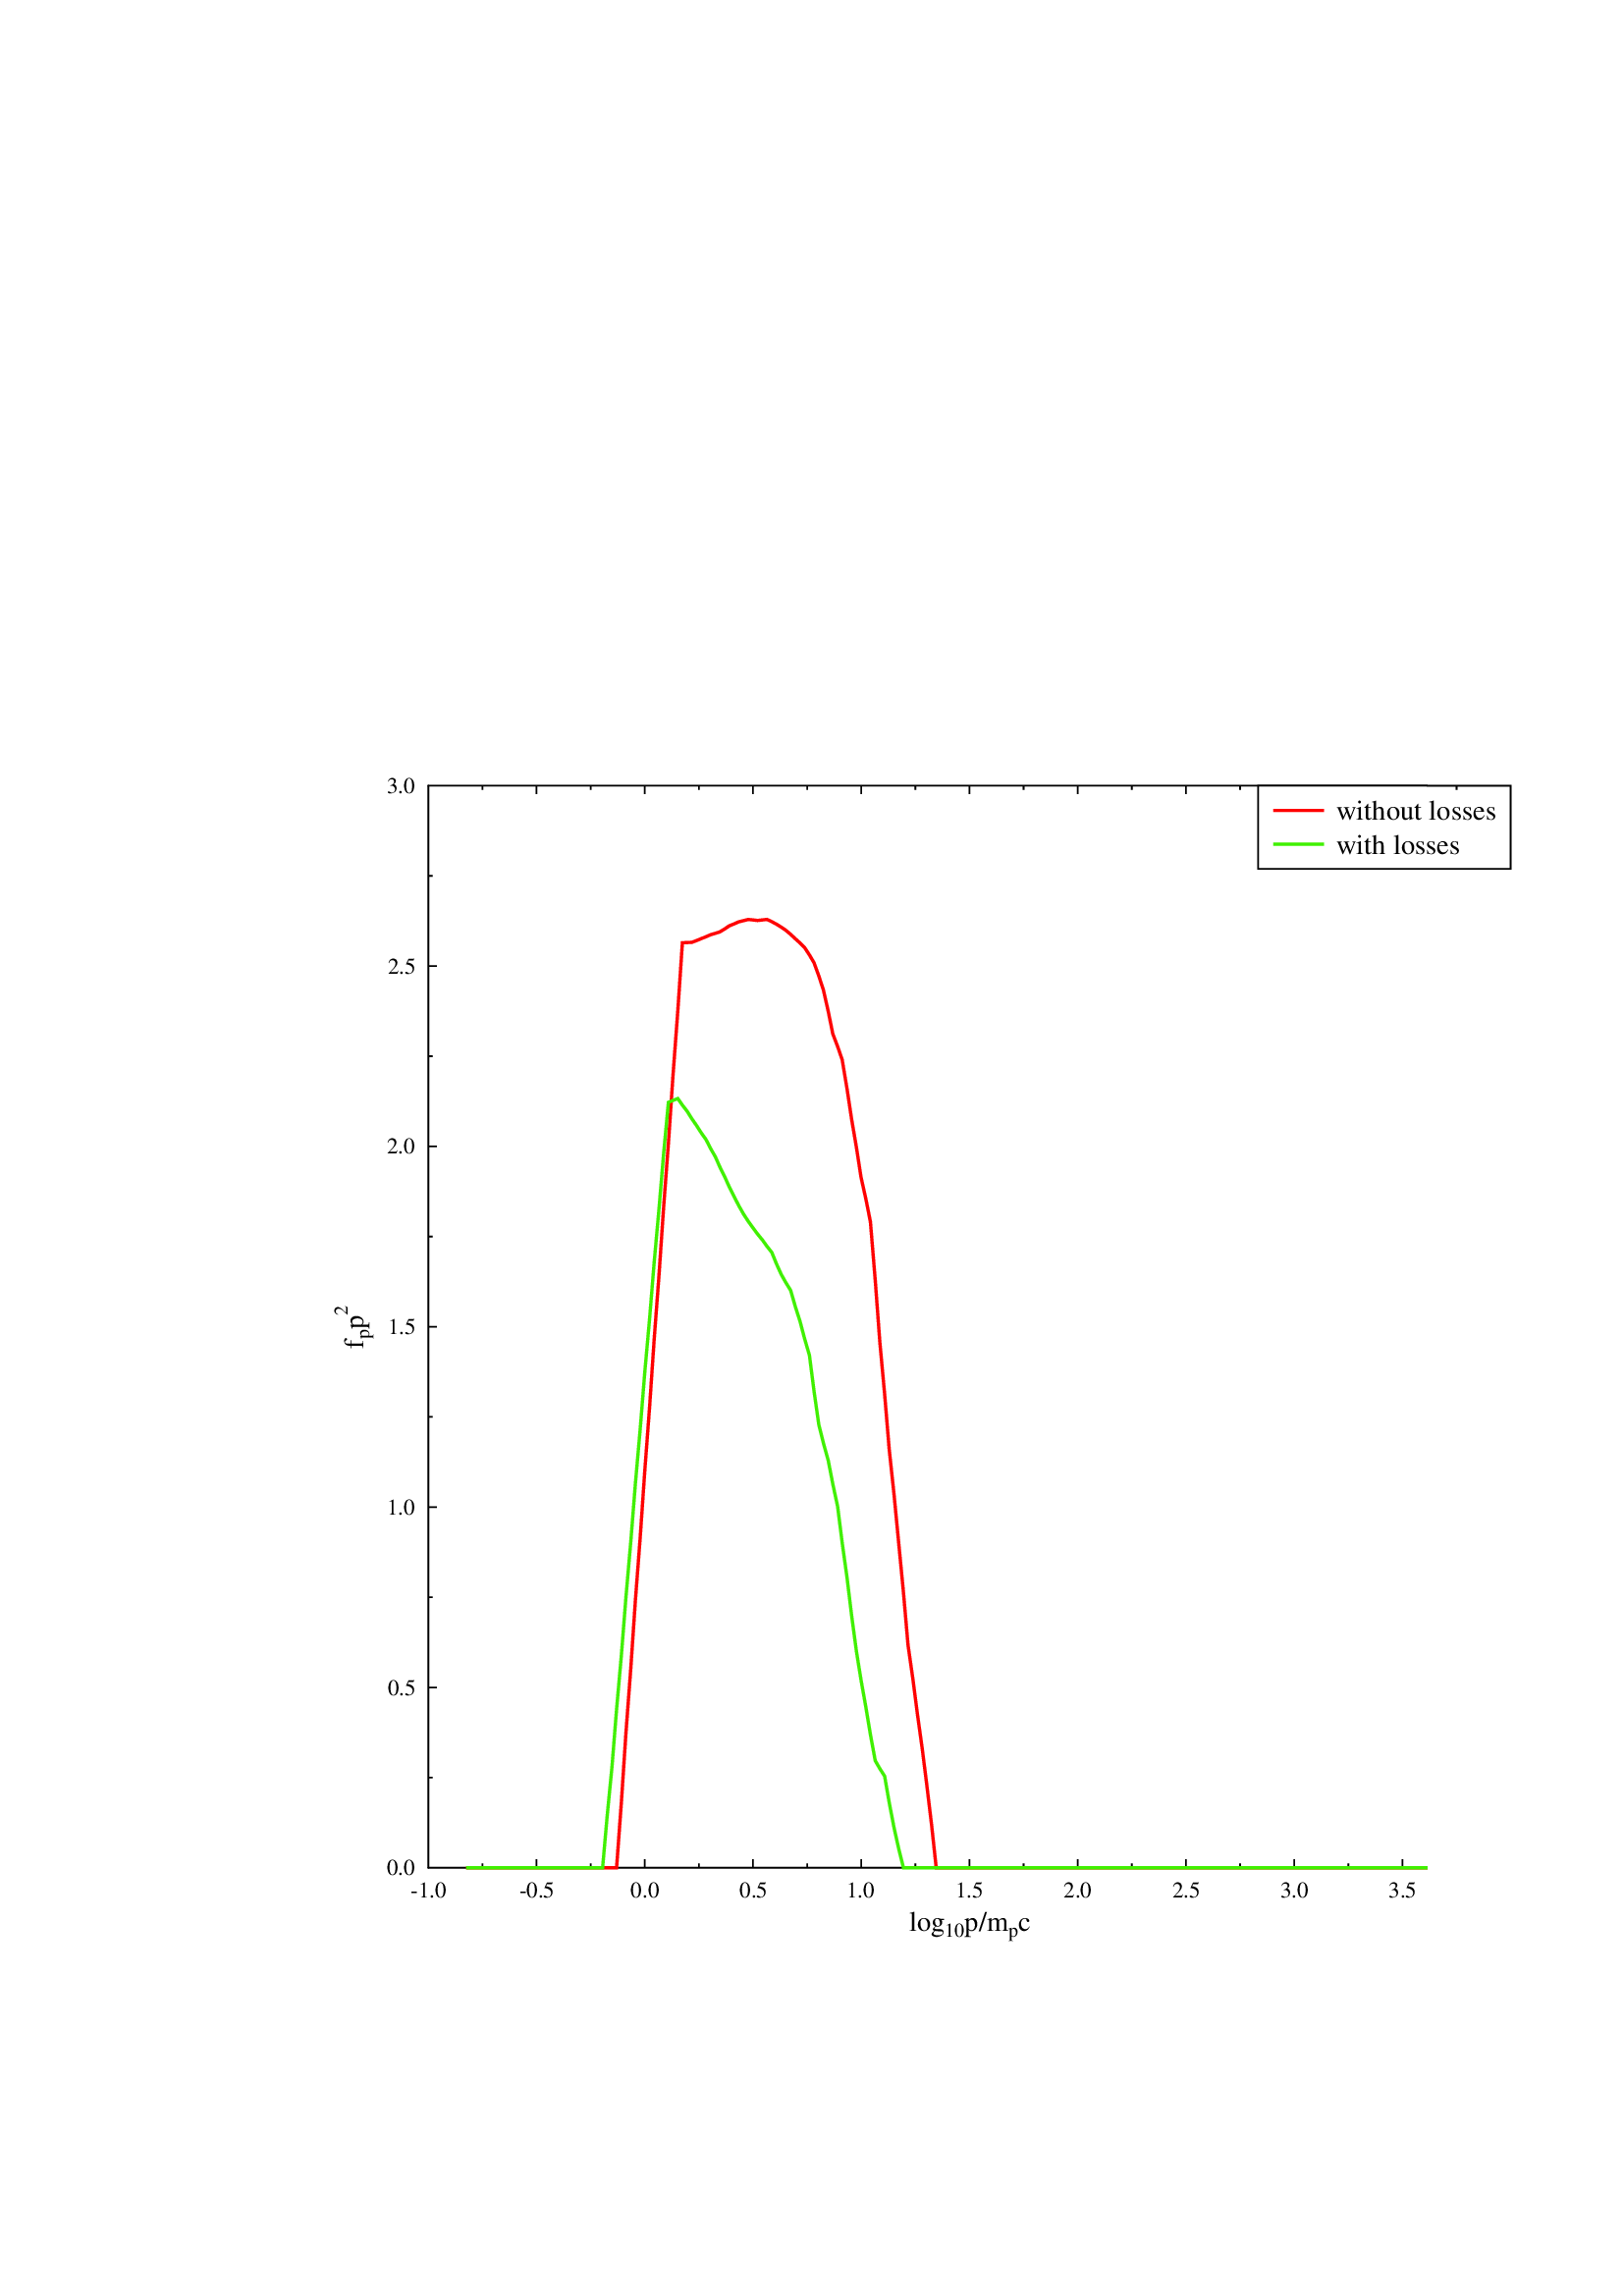
\includegraphics[width=0.90\linewidth]{stoh_sinh_or_not}
\caption{синхротронные потери}
\end{figure}
\end{column}

\begin{column}{0.5\textwidth}
Стохастика
\begin{figure}[H]
\centering
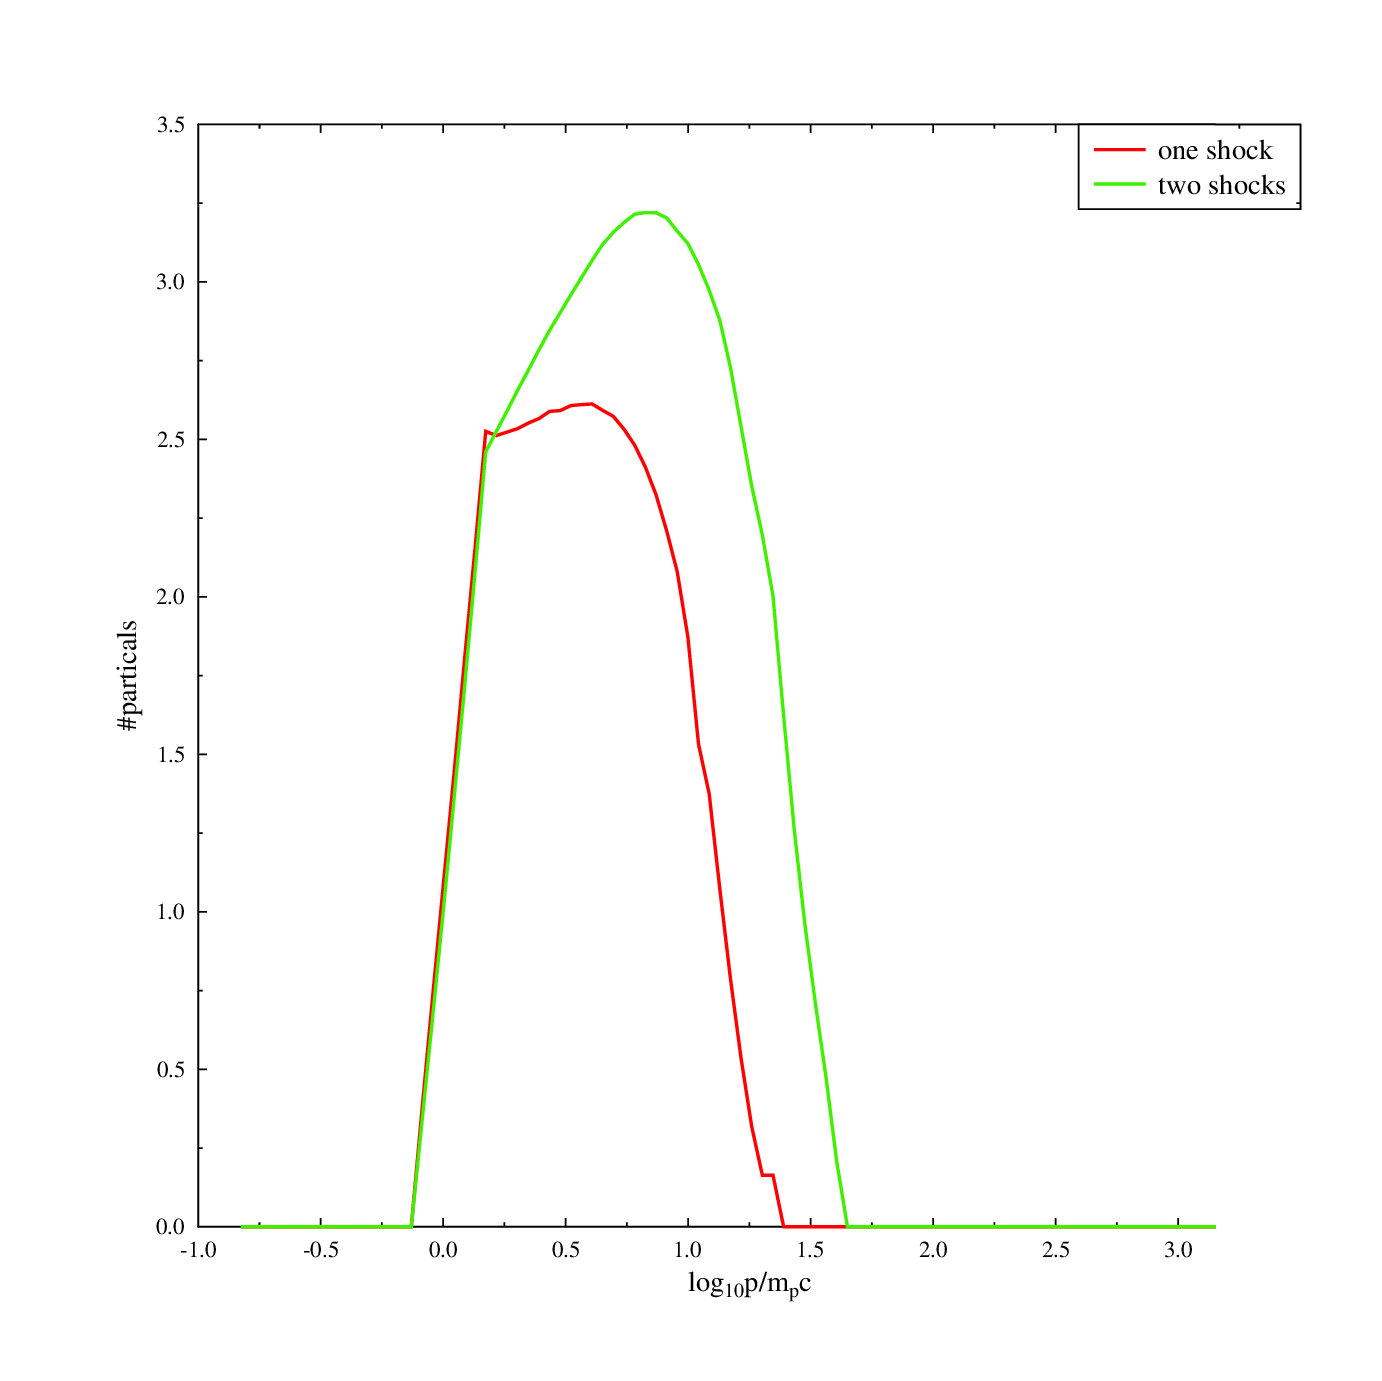
\includegraphics[width=0.90\linewidth]{stoh_two_or_one}
\caption{две волны}
\end{figure}
\end{column}
\end{columns}
\end{frame}

\begin{frame}{Результаты}
\framesubtitle{сравнение}
\begin{figure}[H]
\centering
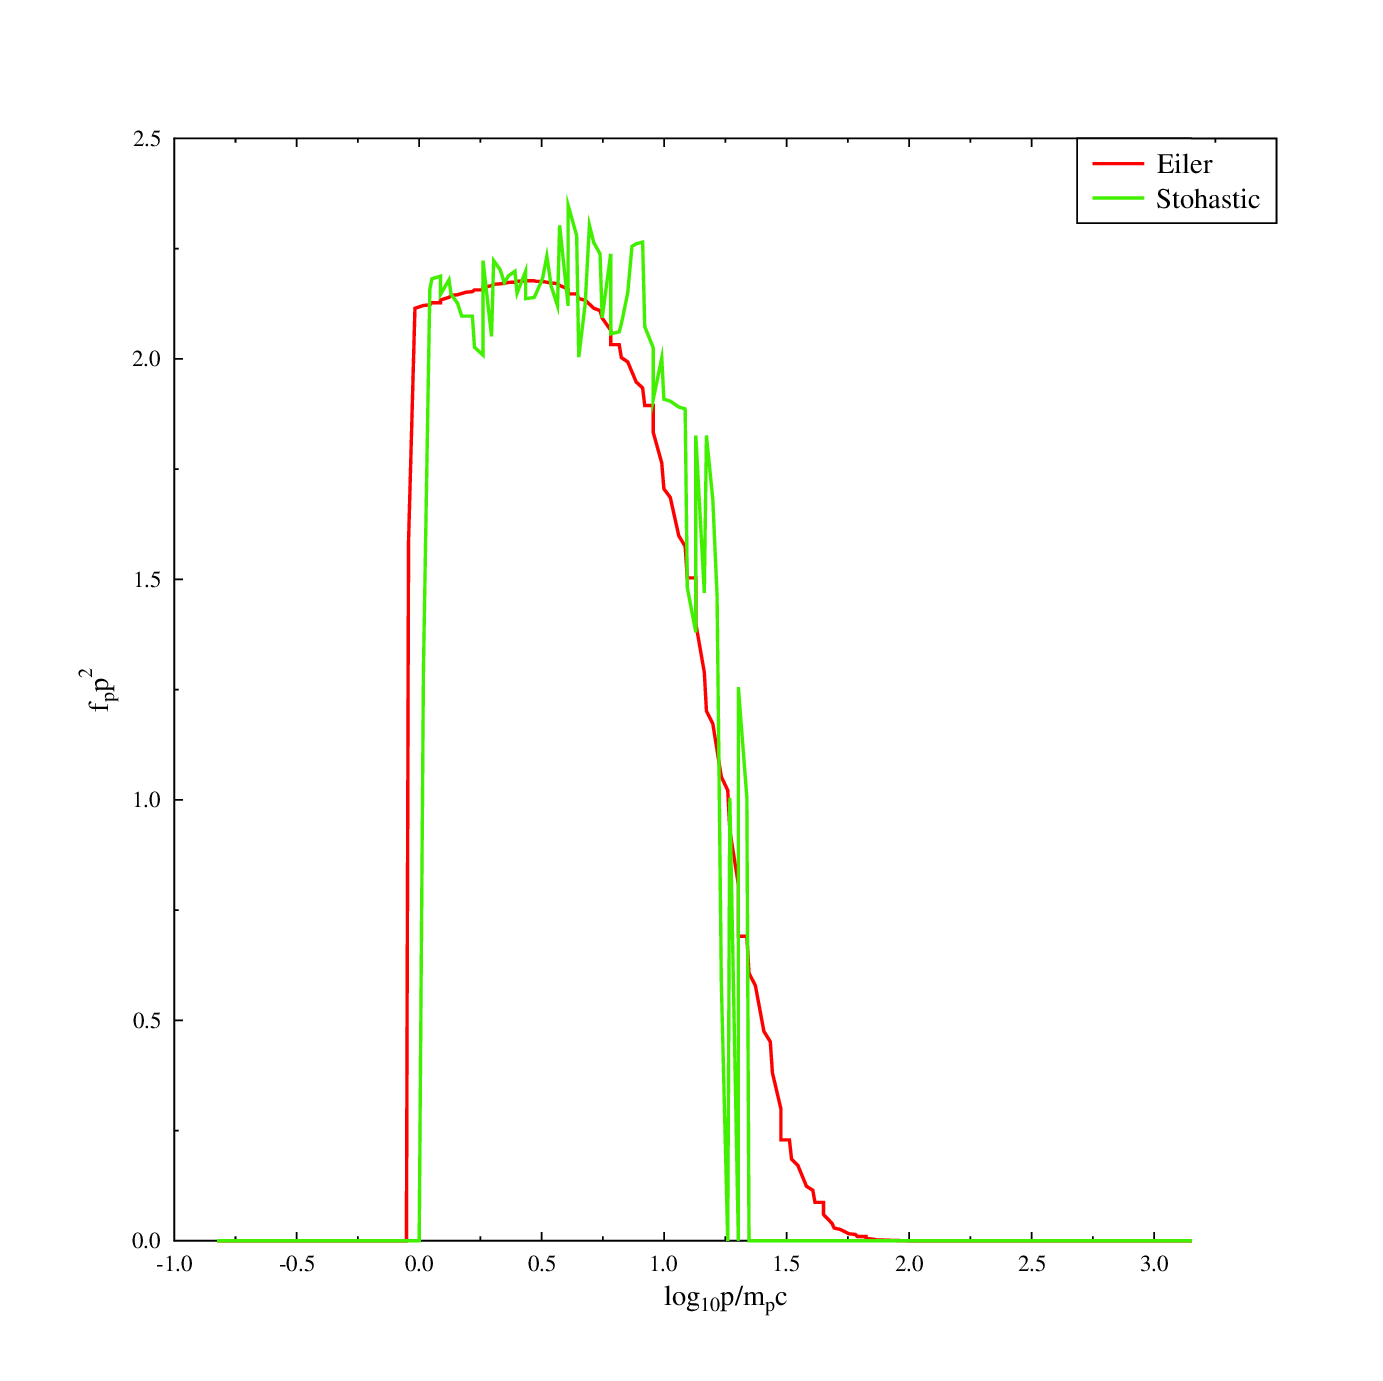
\includegraphics[width=0.3\linewidth]{compare}
\caption{две волны}
\end{figure}

\begin{tabular}{|c|c|c|}
\hline
& Разностная схема & Стохастика \\ \hline
Время & $O(N_tN_pN_x)$ & $O(N_tN)$\\ \hline
Память & $O(N_pN_x)$ & $O(1)$\\ \hline
Параллелизация & по импульсу & по частицам\\ \hline
\end{tabular}
\end{frame}
\section{Выводы}
\begin{frame}{Выводы}
\begin{enumerate}
\item Было получено решение задачи о ускорении частиц на фронте волны с помощью разностной схемы и стохастическим подходом
\item Найдены аналогии между обоими подходами
\item Проведено сравнение подходов
\end{enumerate}
\pause
В обоих подходах есть свои плюсы и минусы, однако по расширяемости стохастический подход проявляет себя лучше подхода с решением с помощью разностных схем.
\end{frame}

\begin{frame}

\begin{figure}[H]
\centering \Large
Спасибо за внимание
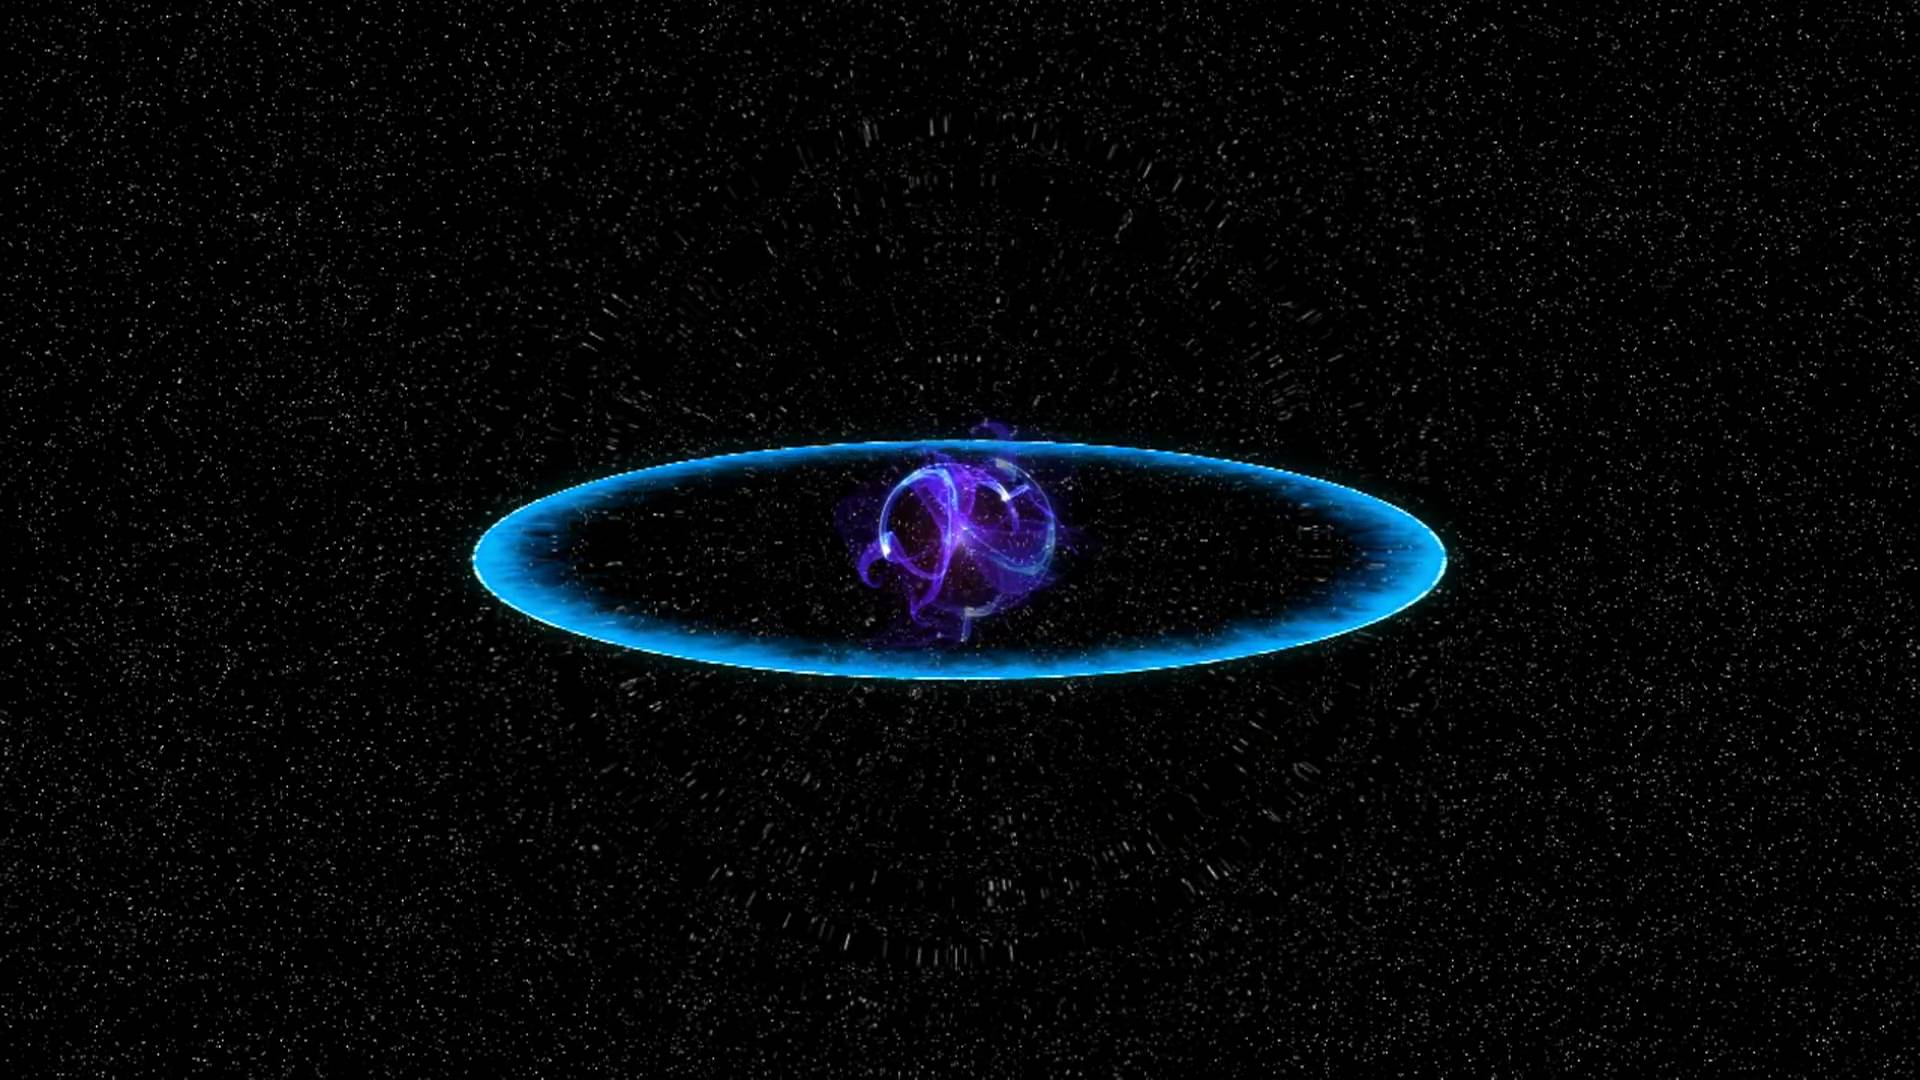
\includegraphics[width=0.8\linewidth]{shock_ill}
\end{figure}
{\small (изображение с \url{http://i.ytimg.com/})}
\end{frame}
\end{document}